\documentclass{beamer}
\usepackage[utf8]{inputenc}
\usepackage[T1]{fontenc}
\usepackage{lmodern}
\usepackage{tabularx}
\usepackage{graphicx}
\usepackage{hyperref}
\usepackage[ngerman]{babel}

\usetheme{Antibes}

\begin{document}
\title{Zwischenpr\"asentation Geek-Shop}
\author{Softwaretechnologie-Projekt 2014 Gruppe 30}
\date{27. November 2014}

\begin{frame}
\titlepage
\end{frame}

\begin{frame}
\frametitle{Gruppenmitglieder}
\begin{tabular}{rp{10cm}}
Chefprogrammierer: & Sebastian Döring \\
Assistent: & Elizaveta Ragozina \\
Sekretär: & Marcus Kammerdiener \\
Tester: & Dominik Lauck \\
Administrator: & Felix Döring \\
\end{tabular}
\end{frame}


\begin{frame}
\frametitle{Inhaltsverzeichnis}\
\tableofcontents
\end{frame}

\section{Entwurfsdiagramme}
\subsection{Entwurfsklassendiagramm}
\begin{frame}
\frametitle{Entwurfsklassendiagramm}
\center{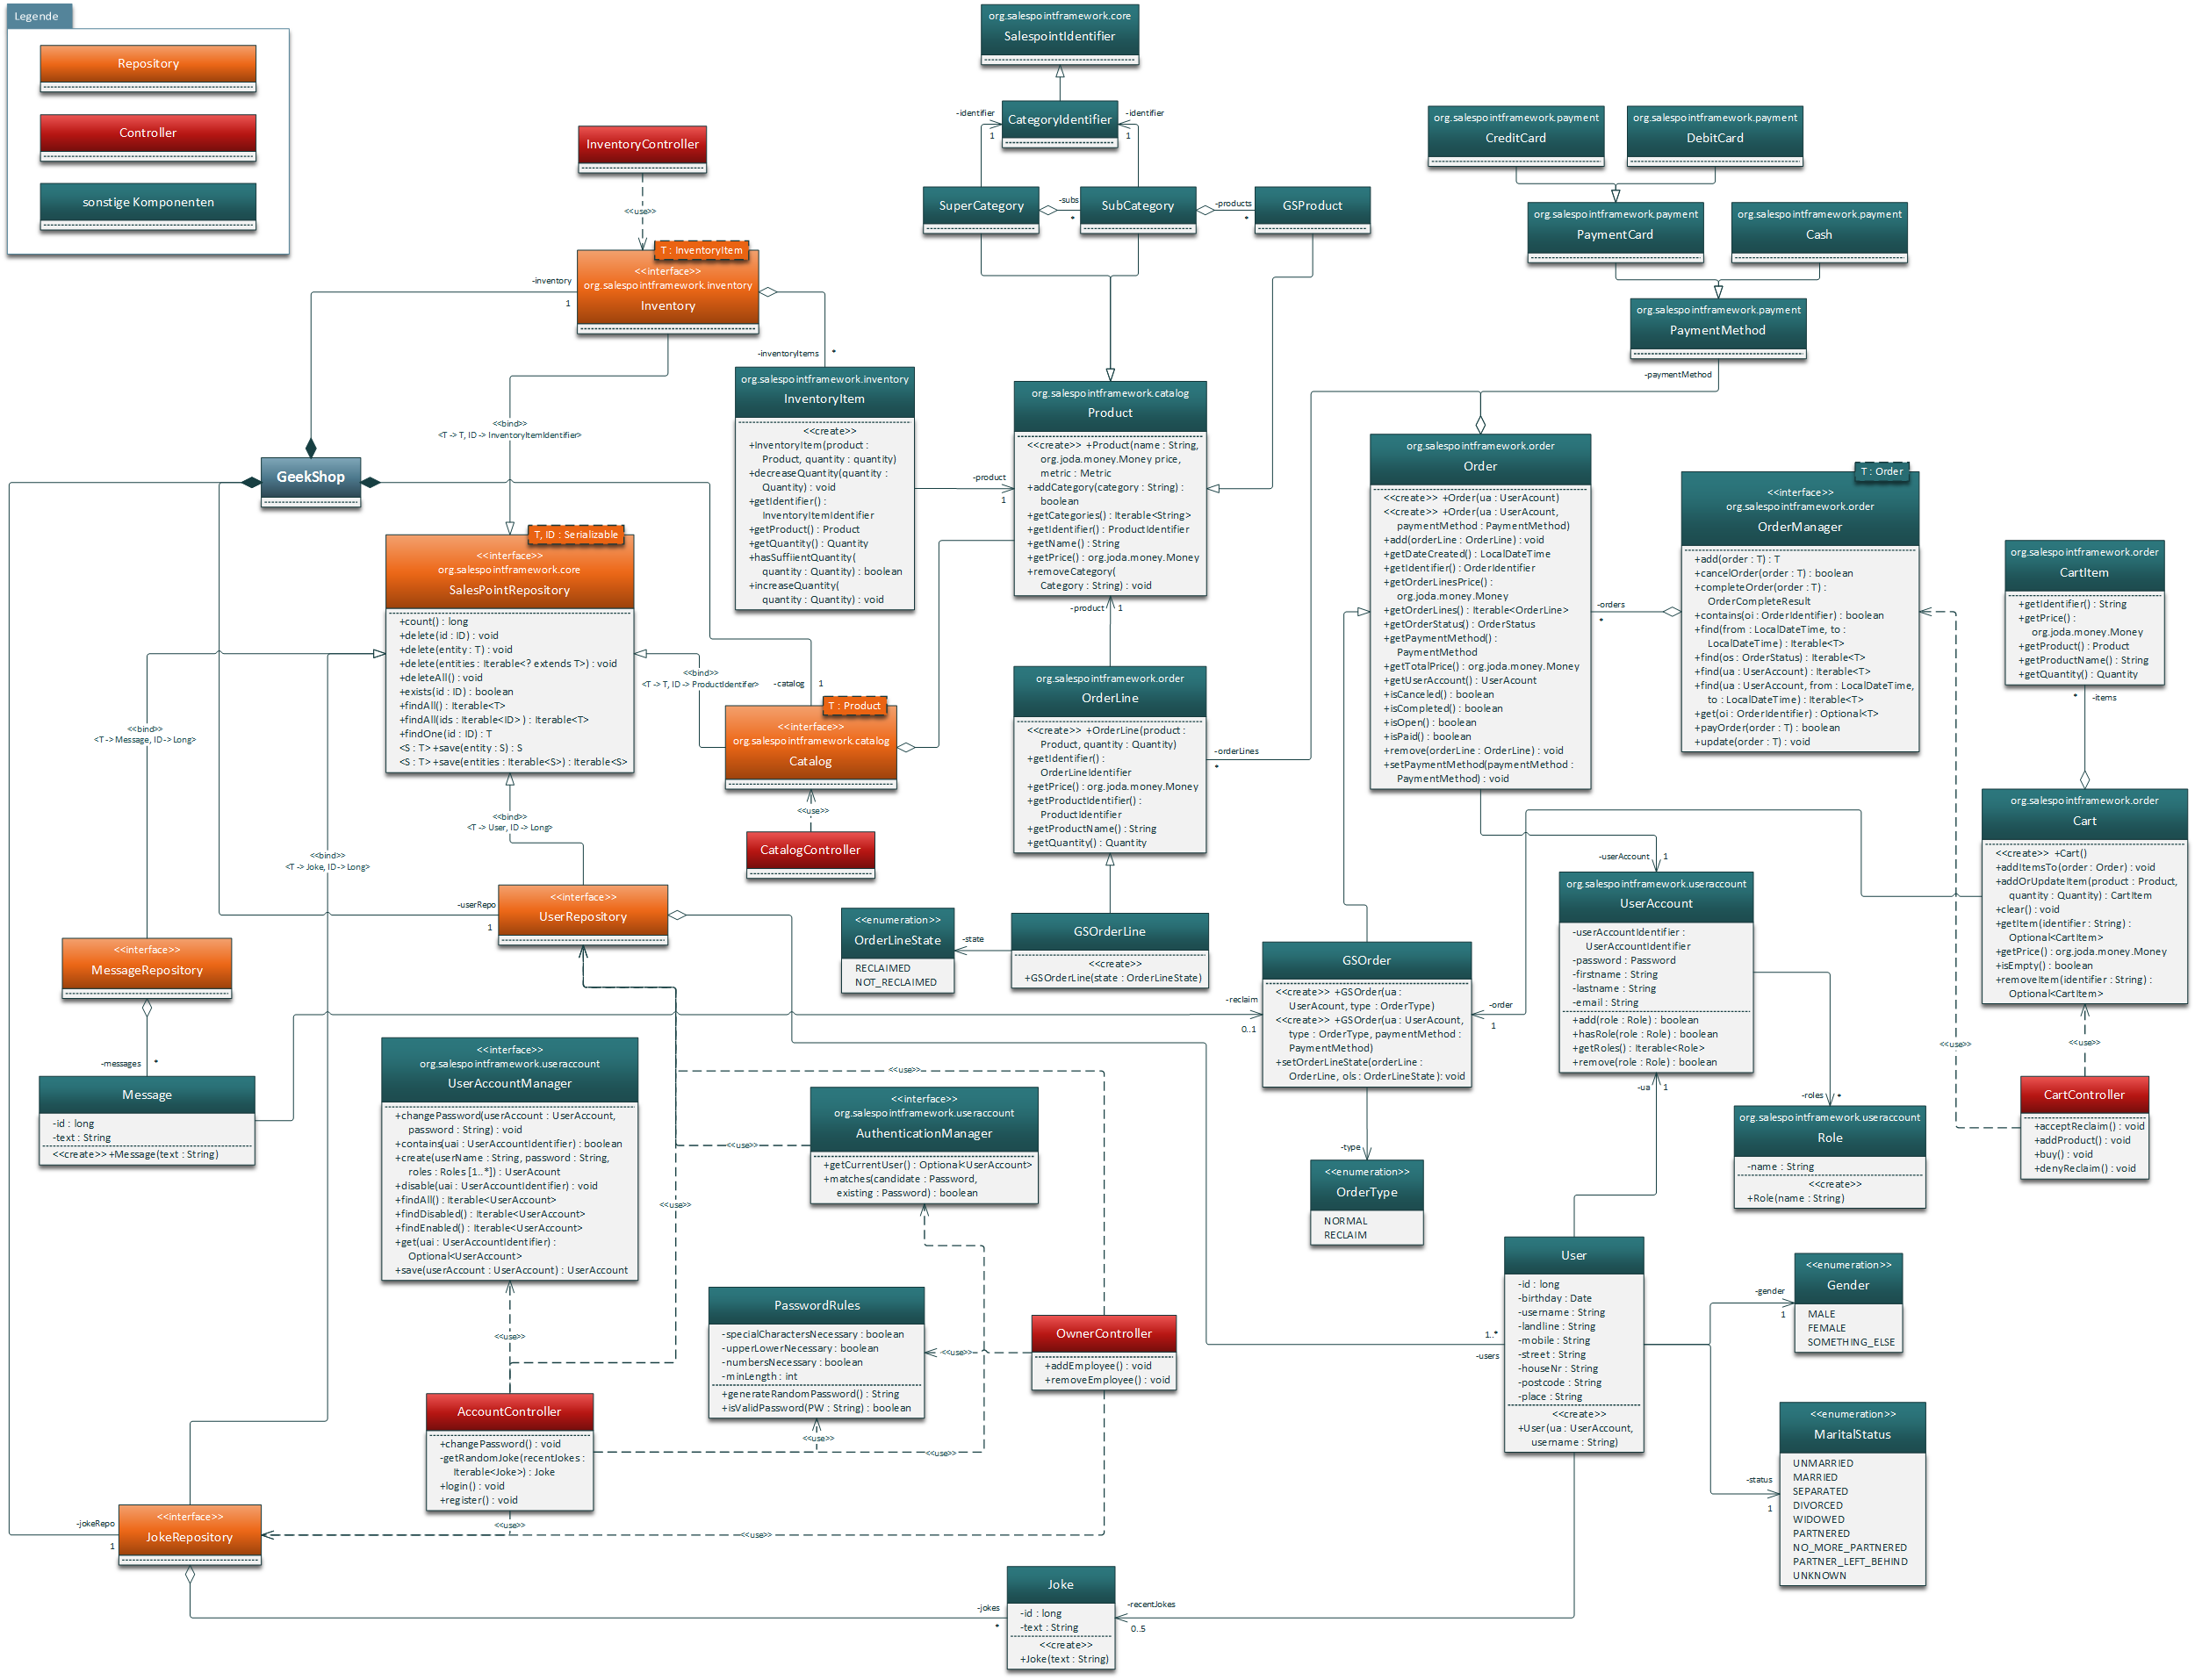
\includegraphics[scale=.13]{../../Entwurf/ekd_ood}}
\end{frame}

\subsection{Sequenzdiagramme}
\begin{frame}
\frametitle{Angestellten hinzuf\"ugen}
\center{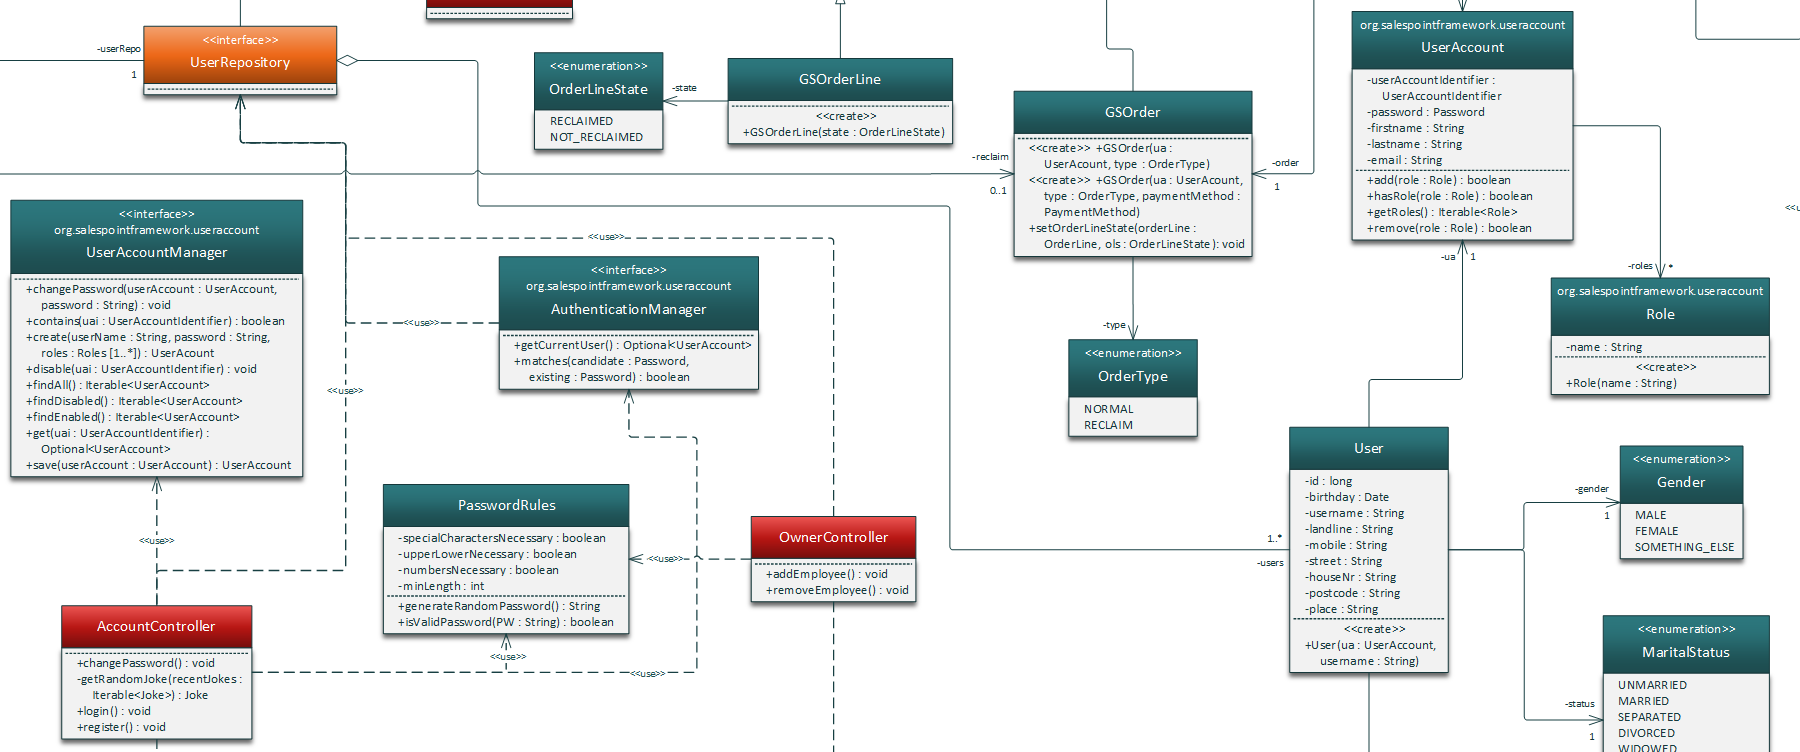
\includegraphics[scale=.3]{source/ekd_user}}
\end{frame}

\begin{frame}
\frametitle{Angestellten hinzuf\"ugen}
\center{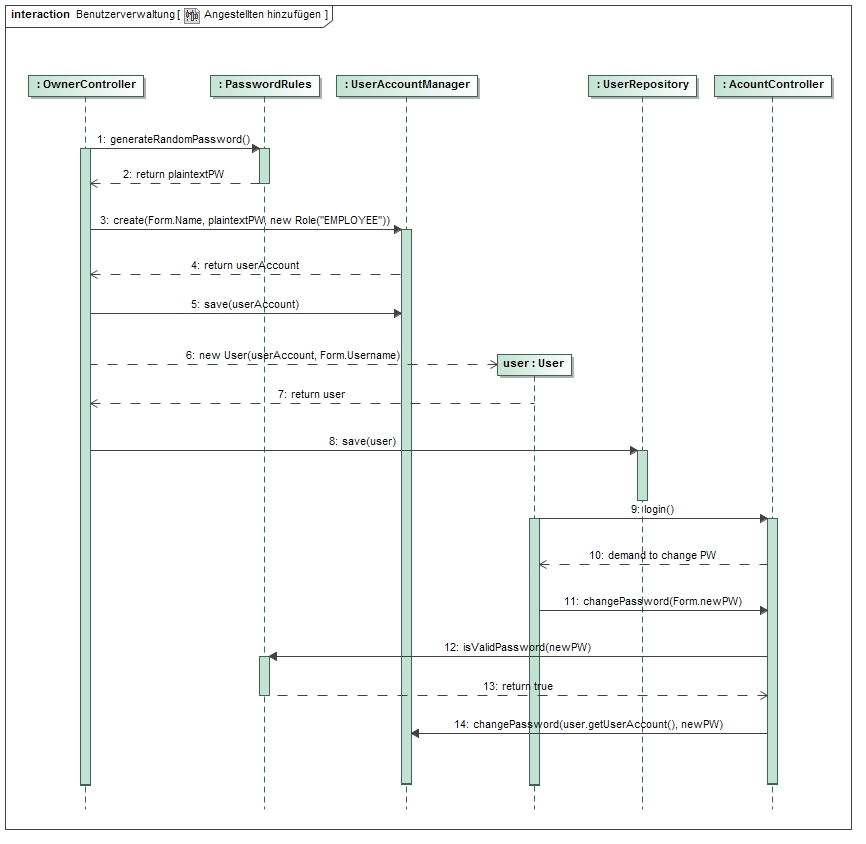
\includegraphics[scale=.25]{../../Entwurf/angestellten_hinzufuegen_ood}}
\end{frame}

\begin{frame}
\frametitle{Kaufvorgang}
\center{\includegraphics[scale=.3]{source/ekd_order}}
\end{frame}

\begin{frame}
\frametitle{Kaufvorgang}
\center{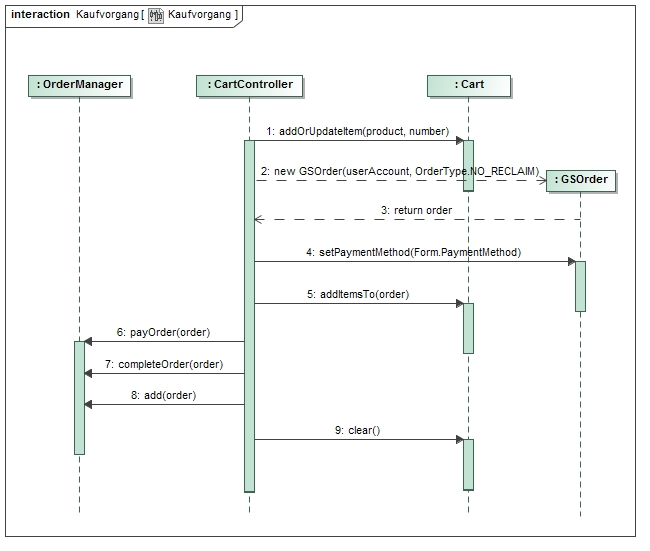
\includegraphics[scale=.25]{../../Entwurf/kaufvorgang_ood}}
\end{frame}

\begin{frame}
\frametitle{Reklamation}
\center{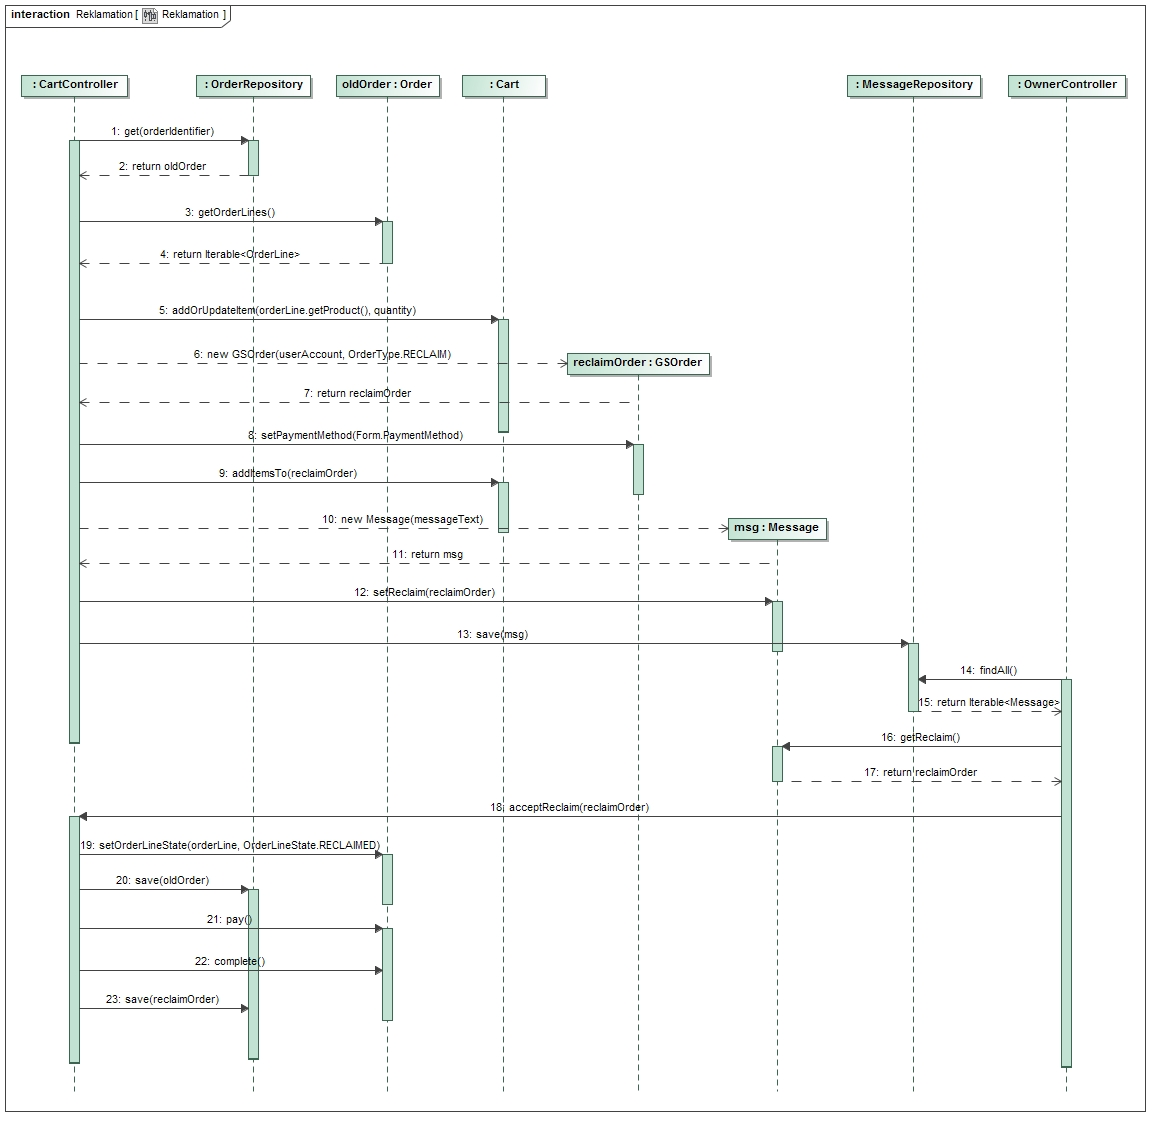
\includegraphics[scale=.25]{../../Entwurf/reklamation_ood}}
\end{frame}

\section{Dialoglandkarte}
\begin{frame}
\frametitle{Dialoglandkarte}
\center{\includegraphics[scale=.3]{../Pflichtenheft/images/dialoglandkarte}}
\end{frame}

\section{Prototyp}
\begin{frame}
\frametitle{Prototyp}
\center{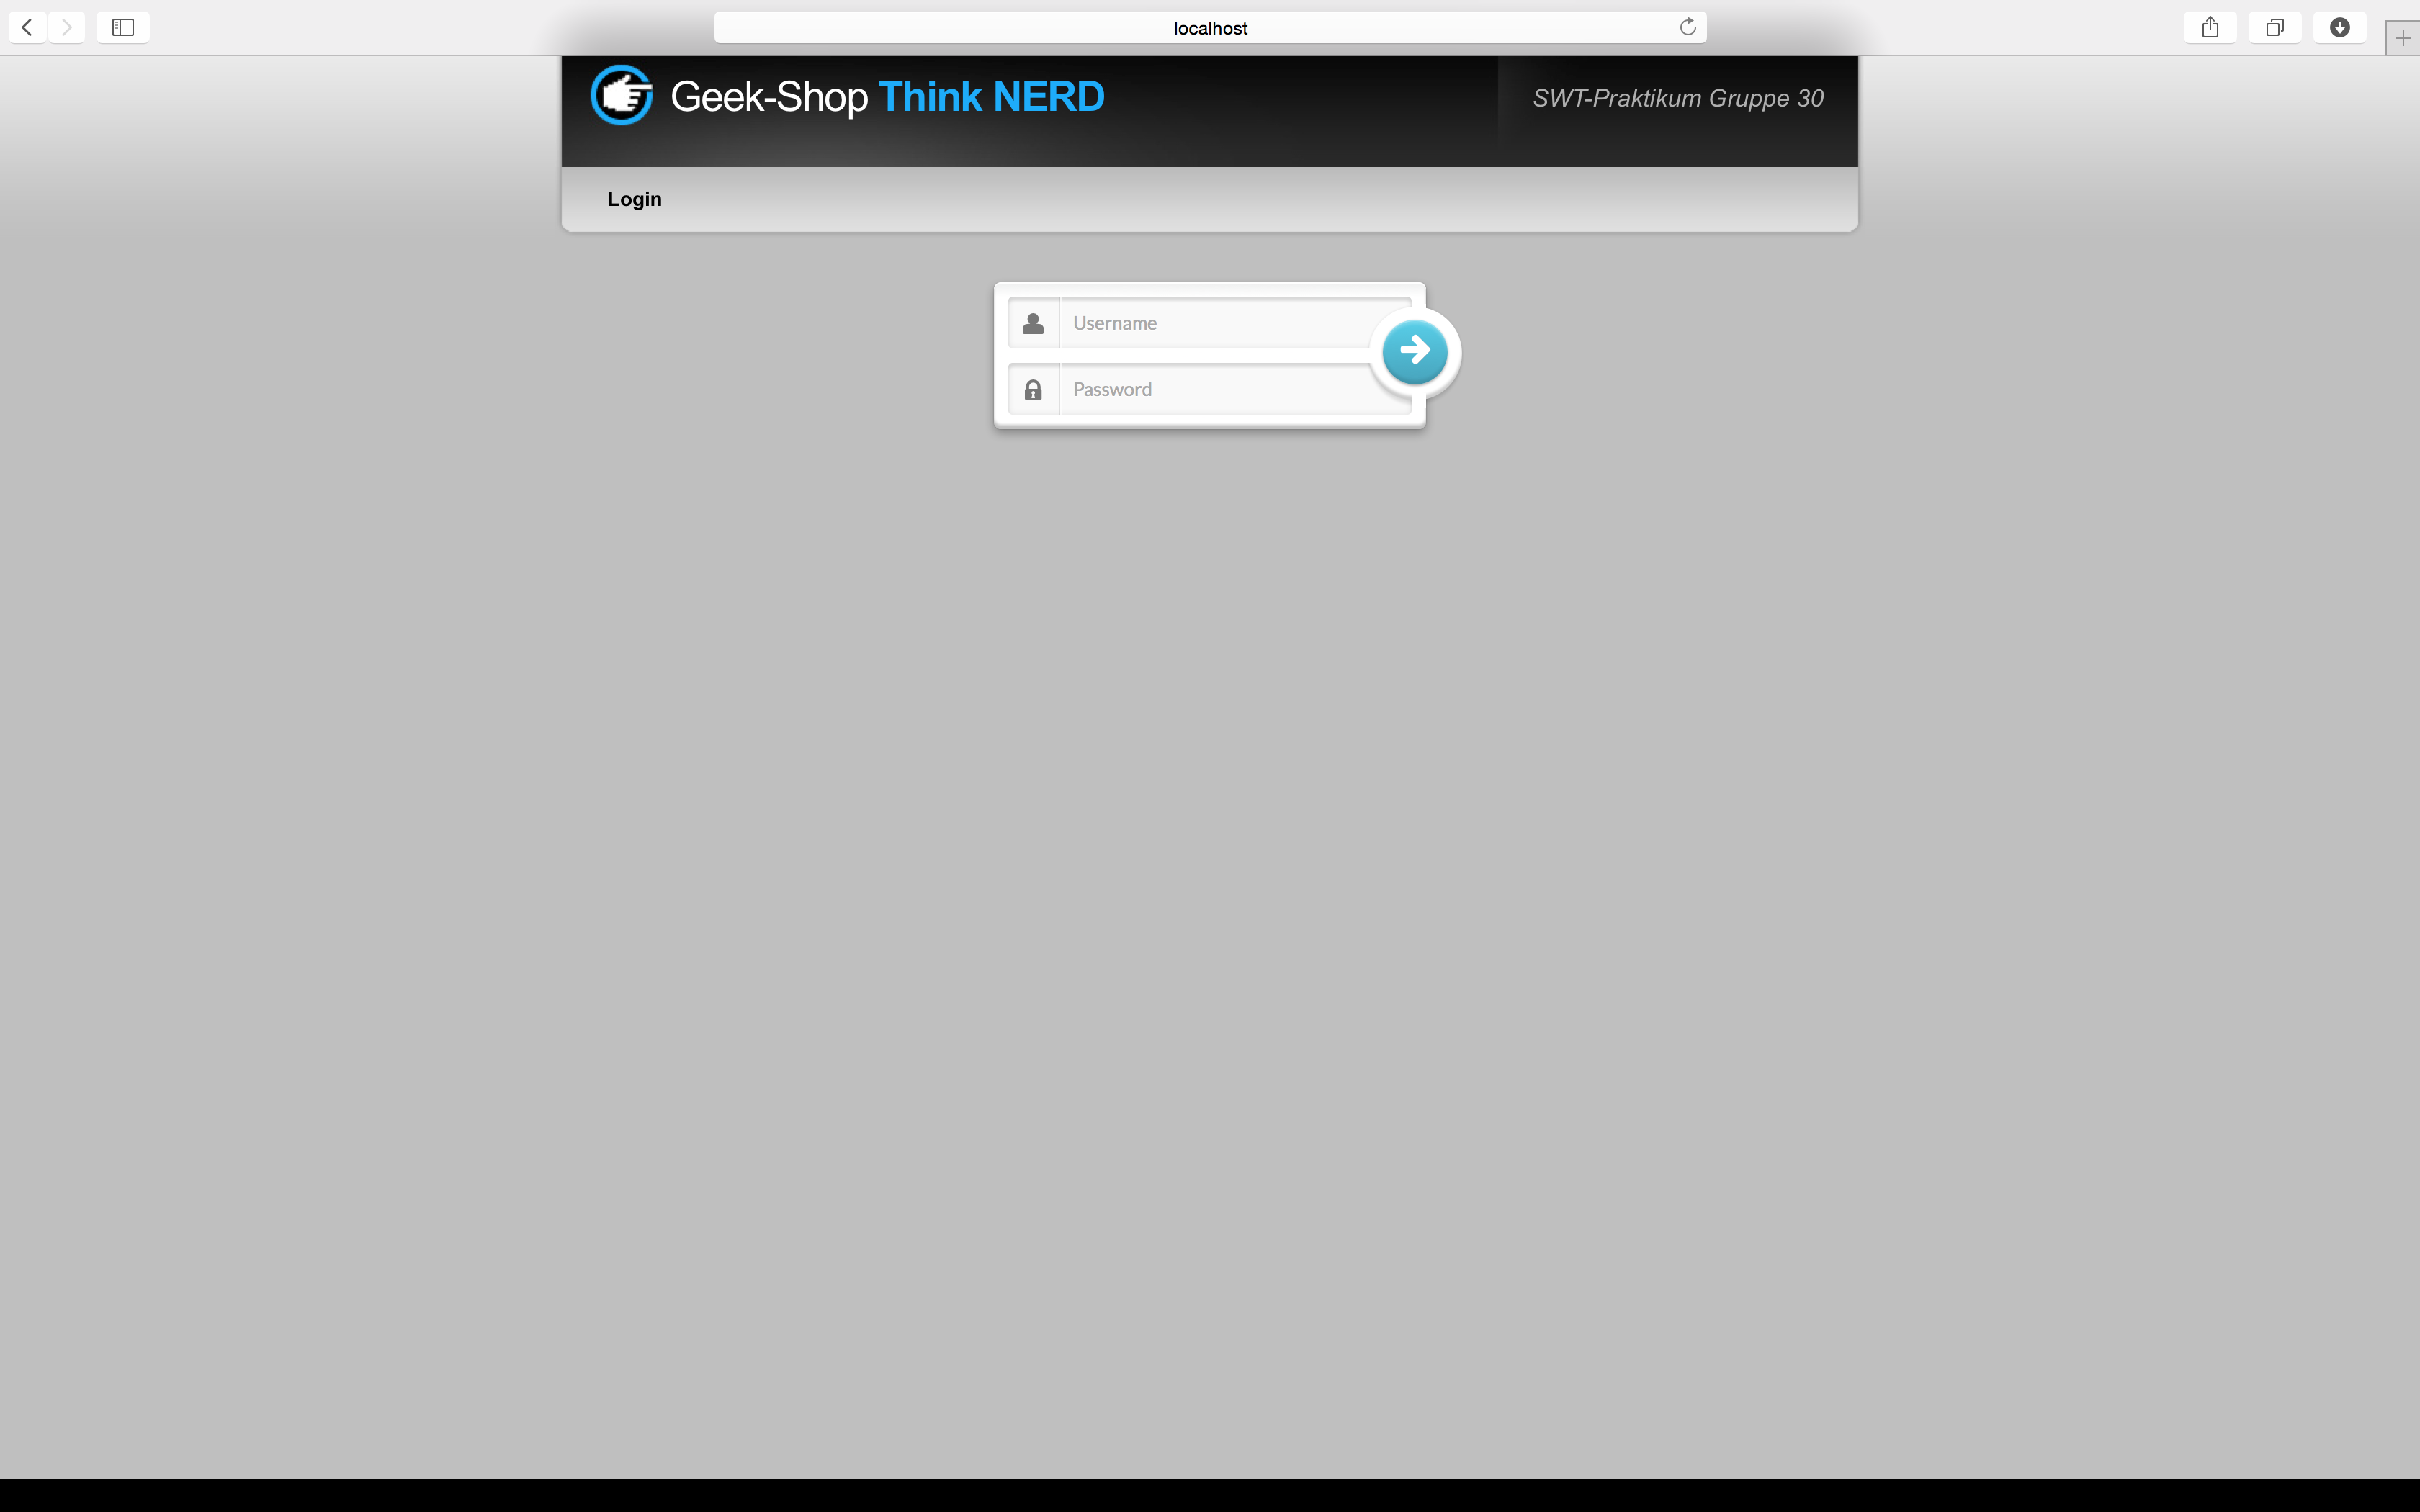
\includegraphics[scale=.15]{source/login}}
\end{frame}

\end{document}
